\documentclass[10pt]{article}
\usepackage[letterpaper,margin=.8in]{geometry}
\usepackage{amsmath,amssymb,booktabs,graphicx,hyperref,xurl}
\hypersetup{hidelinks}\graphicspath{{../figures/}}\setlength{\parskip}{4pt}
\title{S28-0: Finite Affine Operators and Factorial Readiness}
\author{Read-only mechanism audit}\date{23 November 2026}
\begin{document}\maketitle
\section{Outcome and Scope}
Six frozen No-GELU (LA/H3) tokenizers can be materialized as finite affine operators conditional on the shared CNN output. A single shared convolution is insufficient at the two boundary tokens. All six double-precision Source probes pass the predeclared $10^{-9}$ absolute/relative tolerance after explicit boundary handling.

The original runtime uses FP32 tensors with cuDNN TF32 enabled. It fails the unchanged $10^{-4}$ tolerance in all six models and changes one prediction across 12,000 Source packets. A separately preregistered, matched 300-packet TF32-off numerical diagnostic passes. It does not replace the full native-runtime failures or change the historical scientific recipe.

There are zero new scientific fits. The BN-by-GELU fourth cell remains untrained (0/6), and the unchanged source leave-one-RX pilot remains untrained (0/12). The user's attached plan explicitly requires a separate authorization for new fits. Seven synthetic engineering updates are disclosed, including three before a CPU/CUDA comparator error and four after its correction; no RF data enters that gate.
\section{Finite-Length Mathematical Object}
Let $z\in\mathbb R^{32\times8192}$ be the shared CNN output. Each $C_i$ is a finite strided convolution, including its intermediate zero padding and crop. Frozen evaluation BN is the affine map $D_i h+d_i$. Then
\[
T(z)=W_{\rm eff}z+b_{\rm eff},\qquad
W_{\rm eff}=C_4D_3C_3D_2C_2D_1C_1.
\]
The shared CNN contains two BN and two LeakyReLU operations; the RF views and MHA also remain nonlinear. Training BN is batch dependent. Only the tokenizer conditional on $z$ is a frozen affine map.

The convolution (kernel,stride,padding) sequence is $(8,4,2)$ three times, followed by $(4,4,0)$. Lengths are $8192\to2048\to512\to128\to32$. The effective kernel has length 340, stride 256 and padding 42. Its first center is 127.5. The shared CNN extends the nominal local path to 350; global FFT and TrueIB prevent an end-to-end physical locality interpretation.
\[
T(z)_{o,t}=b_{o,t}+\sum_{c=0}^{31}\sum_{q=0}^{339}
K_{t,o,c,q}\,z_{c,256t-42+q},
\]
where outside-input coordinates are zero. Positions $t=1,\ldots,30$ share $K$; positions 0 and 31 need $K_0,K_{31}$. The bias is computed by the original tokenizer's zero response. Local adjoints crop at every intermediate layer; they do not construct a huge dense matrix. All 32 positions remain included. The stored frozen representation has 2,091,008 coefficients, not a model-compression claim.
\clearpage
\section{All Six Frozen Models and Precision Failures}
\begin{center}\small\begin{tabular}{lrrrrr}\toprule
Fold/seed&FP64 token&FP64 logits&Native logits&Native flips&Strict logits\\\midrule
f0\_s201&1.31e-13&5.42e-14&0.01809&0&2.10e-05\\
f0\_s202&9.06e-14&4.62e-14&0.01793&0&2.93e-05\\
f0\_s203&1.46e-13&1.02e-13&0.01869&0&2.15e-05\\
f1\_s201&1.83e-13&5.86e-14&0.02447&0&3.15e-05\\
f1\_s202&1.78e-13&5.97e-14&0.01829&1&2.52e-05\\
f1\_s203&9.06e-14&4.53e-14&0.01796&0&2.09e-05\\
\bottomrule\end{tabular}\end{center}
Errors are maximum absolute differences. Native uses all 2,000 Source-validation packets/model. FP64 and strict-FP32 probes use the first legal validation packet in every TX-by-RX cell: 50/model. Strict here means cuDNN and matmul TF32 disabled; the original native setting is retained in the primary record. Original and converted logits are compared within each setting. No tolerance is relaxed or failing model replaced.
\begin{figure}[htbp]\centering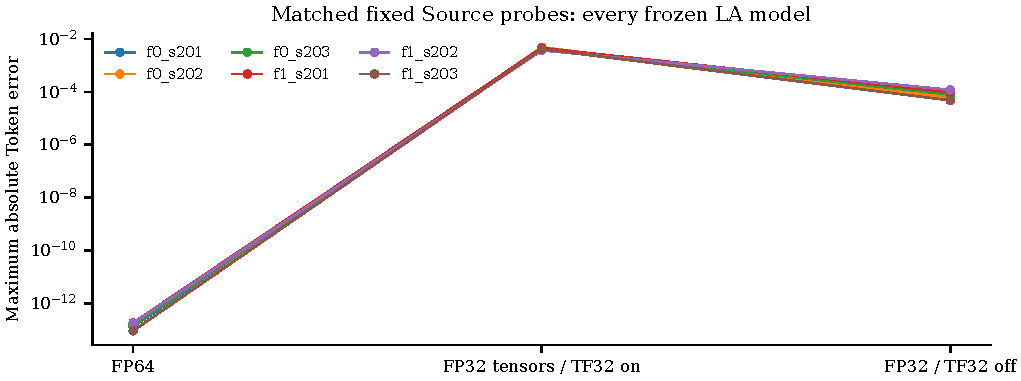
\includegraphics[width=.97\linewidth]{precision.pdf}
\caption{Matched 300-packet Source probes, all six models. These are numerical differences of frozen functions, not training-performance changes.}\end{figure}
\begin{figure}[htbp]\centering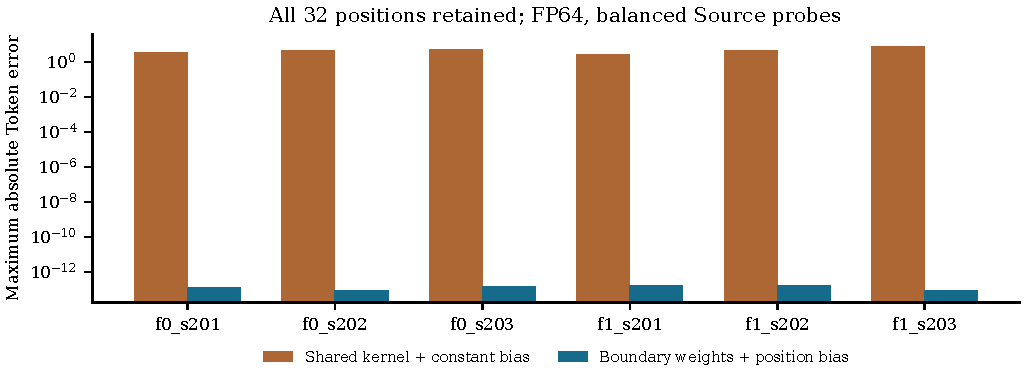
\includegraphics[width=.97\linewidth]{boundaries.pdf}
\caption{The shared-kernel baseline fails at the boundaries. Explicit boundary weights and position bias restore the double-precision finite operator.}\end{figure}
\clearpage
\section{BN by GELU: A Registered Missing Cell}
\begin{center}\small\begin{tabular}{lccrrr}\toprule
Cell&Mid BN&GELU&Params&Historical Dev&Source val.\\\midrule
H0&yes&yes&133,690&97.335&98.175\\
LA&yes&no&133,690&96.583&97.742\\
H2&no&yes&133,338&96.145&97.142\\
H2\_LA&no&no&133,338&not run&not run\\\bottomrule\end{tabular}\end{center}
\[
\Delta_{BN\times GELU}=(A_{H0}-A_{LA})-(A_{H2}-A_{H2\_LA}).
\]
The interaction is not estimated while its fourth cell is missing. Exactly six new H2\_LA fits are planned; eighteen original factorial models are reused and six LP models are secondary controls. Only the three intermediate BN and three GELU modules become Identity. H2 and H2\_LA have the same full initial state; all surviving values match H0 for each paired fold/seed. Two shared-stem BN modules remain. Removing middle BN also removes 352 affine parameters and changes batch statistics, running statistics and optimization jointly.

The exploratory plan follows the original two folds, seeds 201/202/203, first 160/last 40 packets/TX/RX, 200 epochs, batch 64, AdamW, AWGN and minimum clean Source RX-equal CE. All six new models must be sealed before common Dev reporting. Ten unique RXs are resampled after averaging seeds within RX (10,000 repetitions, seed 28028). The two-sided practical rule requires magnitude at least .5pp, conditional 95\% interval excluding zero, at least 5/6 paired effects and both fold means in the same direction. Failure to meet the rule establishes neither equivalence nor absence of a BN effect. The design follows historical Dev observation and is not independent confirmation.
\section{Independent Source-Held Pilot, Still Inactive}
The original S27-C JSON is preserved byte for byte. Fold 0 trains rtl1/rtl3/rtl6/rtl9 and holds b210\_1; fold 1 trains b200\_mini\_1/pluto\_1/rtl2/rtl7 and holds rtl\_5. Twelve fresh H0/LP models use the fixed S27C-H4x160 paired initialization, never the five-RX-trained weights. Each fit has 6,400 training packets, 1,600 Source-validation packets, 100 updates/epoch and 20,000 total updates. Only four-RX validation selects checkpoints; held evaluation waits for all twelve models to be sealed.

Report both absolute accuracies and $\Delta G=(A_{S}-A_{H})_{H0}-(A_{S}-A_{H})_{LP}$. Retain the original rule: held H0-minus-LP at least .5pp and $\Delta G\leq-.5$pp in both receiver/fold means, with at least 5/6 jointly favorable fit pairs. Two held RXs do not become six independent receivers; no population-RX bootstrap or significance is justified. A held-only distribution has one RX: its across-RX scatter is zero by construction, so $J_c$ cannot identify receiver invariance. That diagnostic must be marked not identifiable, rather than interpreted using an epsilon ratio.
\clearpage
\section{What Is and Is Not Established}
The function representation motivates studying structured parameterization and training paths. It does not identify an optimization cause. LA retains batch-dependent training BN; LP differs in grouping, freedom, initialization and compute. Removing all middle BN/GELU is a distinct six-fit intervention, not a proof that the complete RF network is linear.

A free dense 32-to-64, length 340 convolution already has 696,384 kernel/bias parameters, versus 86,256 for the four convolution factors without BN. Allowing independent boundary kernels changes capacity further. Equal starting predictions do not equalize parameter constraints or AdamW states. A future direct-operator optimization control needs a separate audited design; no S28-B search or fit is started.

The evidence matrix retains every previous S27-B entry and adds the qualified affine representation. BN-by-GELU interaction, RX-specific gap reduction and a unique optimization explanation remain untested. Neither MHA amplification nor a monotonic Source $J_w$ explanation is reinstated. No new independent acquisition, blind RX or physical receiver invariance is established.
\section{Integrity and Execution Boundary}
All 24 historical models strictly recover their original Source metrics over 48,000 predictions. Model, configuration and 200-epoch history hashes remain unchanged; minimum-Source-CE selection is verified. The mathematical contract and data permissions were committed before Source IO. After native precision failures were recorded, the supplemental matched precision diagnostic was separately frozen and committed before execution. It preserves the six native failures and the one changed prediction.

This audit reads historical five-Source validation, including RXs later designated held in C. It does not create a new C model or a C held evaluation, and never claims these physical receivers have no research exposure. There are no new Dev, Confirm or blind packets. Synthetic engineering updates are counted separately; the corrected optimizer comparator compares exact dtype/values across CPU/CUDA scalar placement without changing the recovery implementation.

The scientific fitting budget is zero. The training entry rejects execution until an explicit user authorization and committed activation. Architecture, initialization, mathematical composition, resources, roles and resume checks have passed; scientific A/C cohorts have not been executed. Raw waveforms and converted coefficient tensors remain local. Public code, plans, complete error tables, logs and audit records support reproduction. The Chinese report contains the detailed evidence boundaries and exact plan links.
\end{document}
